The background modeling are strategies used to model the backgrounds that matches the data distribution in the control region. The main sources of SM background in this analysis can be divided into 3 groups:
\begin{enumerate}
\item Zjets events: Zjets process is the dominating background source for this search, with $\ell$ in the final state from the Z decay. ${p_{T}}^{miss}$ is only instrumental.
\item Non-resonant events: Events that have $\ell$ and ${p_{T}}^{miss}$ in the final state, but $\ell$ pair does not come from the decay of a resonance. $t\bar{t}$ and $WW$ processes are the main sources of the non-resonant background
\item Resonant event: Events that have $\ell$ and ${p_{T}}^{miss}$ in the final state, while $\ell$ pair comes from the decay of a Z boson. $ZZ$ and $WZ$ are the main sources of the resonant background
\end{enumerate}

\vspace{0.3cm}
The background modeling starts from tuning the MC simulation samples. MC simulation is widely used in this analysis. The modeling of the resonant background and the signal completely rely on MC simulation. Though the modeling of the Zjet and non-resonant background are done by data-driven methods, simulation samples are also used in the process. Various weights are asigned to the MC events to compensate the discrepancies between the simulation settings and the actual experiment, in terms of pileup, HLT and lepton ID/Iso. Then the detail of the background strategies for the 3 background groups are discussed.

\section{Pileup re-weighting}
The number of pileup interactions is directly related to the contamination in an event, and can affect the quality of the event reconstruction, such as the value of ${p_{T}}^{miss}$ and lepton isolations. For the MC events, a random number of pileups are added during their production, which does not necessarily agree with the pileup distribution in the data. To align the distribution of pileup numbers between data and simulation, pileup re-weighting is applied to the MC samples. 

\vspace{0.3cm}
Considering the reconstruction efficiencies of the vertices might differ between MC and data, a safe way is to reweight based on the distribution of the number of actual pileup interactions (true pileup), rather than observed interactions. And the value of the weight assigned to the MC events would be obtained from the ratio of true data pileup profile and true MC pileup profil. The true MC pileup profile can be found in the configuration of the RunIISummer16 MC production. The true data pileup profile can be calculated based on the instantaneous luminosity for each bunch crossing noted in the CMS pileup JSON file, and the recommended Mini-Bias cross-section of $69.2 mb \pm 4.6\%$ evaluated by the CMS luminosity POG.

\vspace{0.3cm}
Figure~\ref{fig:bg_pileup} shows the distribution of the true pileup number for both data and MC, as well as their ratio. The pileup reweighting value for each event in the MC samples are obtained from the ratio plot based on the true pileup number in that event.

\begin{figure}[htbp]
\begin{center}
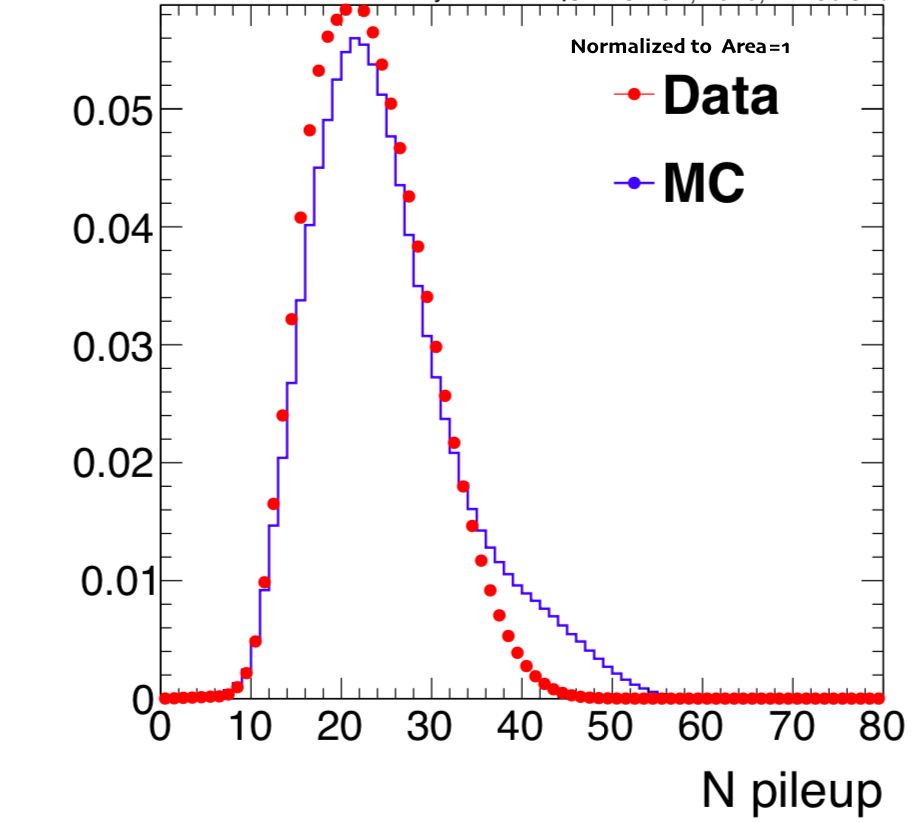
\includegraphics[width=0.9\linewidth]{figures/bg_Npileup.png}
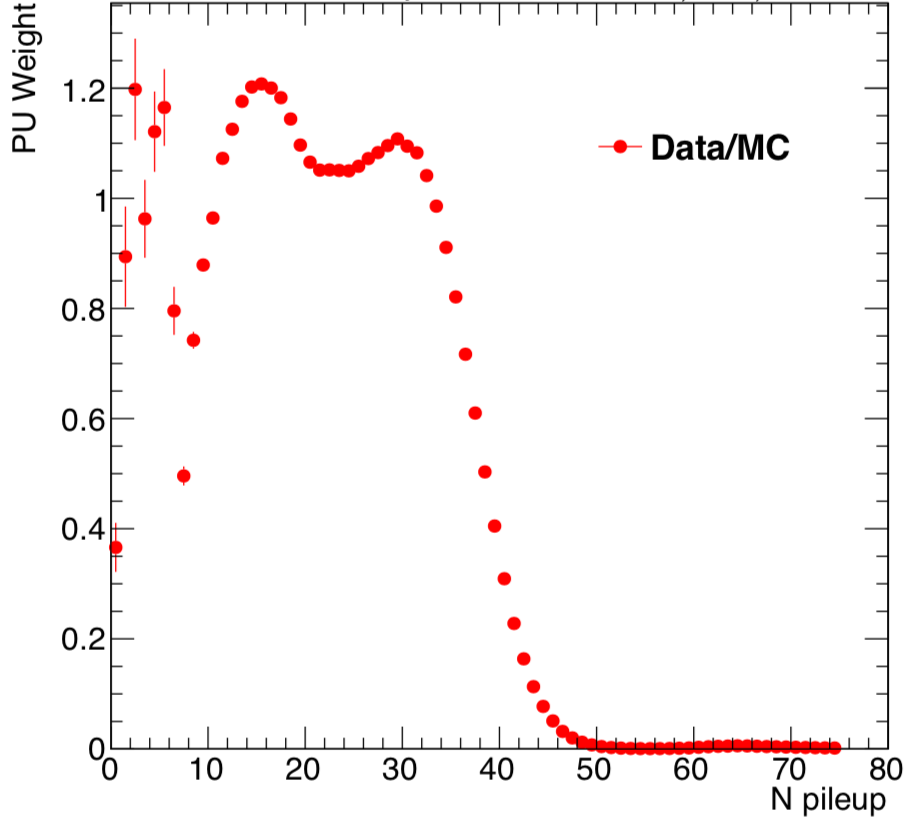
\includegraphics[width=0.9\linewidth]{figures/bg_pileupratio.png}
\caption{Pileup number profiles (left) for RunIISummer16 MC and 2016 data; and the pileup re-weighting function (right).}
\label{fig:bg_pileup}
\end{center}
\end{figure}

\section{Monte Carlo Efficiencies}
Weights are also applied to the MC samples in terms of the discrepancies in HLT, lepton ID/Iso efficiencies between data and MC samples. The chance of a lepton passing HLT, ID and Iso should be:
\begin{equation}
P(HLT\cdot ID\cdot Iso) & = P(HLT|ID\cdot Iso)\times P(ID\cdot Iso) \\
& = P(HLT|ID\cdot Iso)\times P(Iso|ID)\times P(ID)
\end{equation}

where $P(HLT\cdot ID\cdot Iso)$ denotes the efficiency of a lepton passing HLT, ID and Iso; $P(HLT|ID\cdot Iso)$ is the efficiency of a lepton passing HLT under the condition of it passing ID and ISO, and is also referred to as trigger efficiency; $P(ID\cdot Iso)$ is the ID/Iso efficiency; $P(Iso|ID)$ is the efficiency of a lepton passing Iso under the condition that it passes ID, and it is also referred to as the Iso efficiency; $P(ID)$ is the ID efficiency. The efficiencies are all calculated using a Tag-and-Probe method in this analysis, as discussed below. 

\subsection{Muon ID/Iso Efficiency}
The ID/Iso efficiencies may differ between MC and data due to detector effect. Therefore efficiencies are measured and scale factors (SF) are calculated for the MC samples to counter this effect. The Muon High $p_T$ ID, Tracker High $p_T$ ID and the Tracker Isolation efficiencies are measured separatedly using the tag-and-probe method discribed as below. Events are selected from the SingleMuon dataset for data and DYJetsToLL\_M-50\_TuneCUETP8M1\_13TeV-madgraphMLM-pythia8 dataset for MC with pileup reweight. 

\vspace{0.3cm}
In the tag-and-probe method, a tag muon and a probe muon are selected from a event. The tag muon is a muon known as well-defined, which helps eliminate bias and calculate efficiency, and the probe muon is the muon candidate from which the efficiency is studied. A event is kept only if two muons are found with one passing the "tag" criteria while the other passing the "probe" criteria. For the muon ID/Iso efficiency measurement, the tag criteria are:
\begin{enumerate}
\item passing the \texttt{tight} Muon ID and the $relIso<0.2$ Iso requirment recommended by CMS Muon POG
\item passing \texttt{HLT_IsoMu24} and $p_T > 26 GeV$
\end{enumerate}

The ID and Iso requirment ensures the tag muon to be a well defined muon. The \texttt{HLT_IsoMu24} is the un-prescaled HLT with lowest $p_T$ threshold in the SingleMuon dataset. Requiring the tag muon to pass this HLT assures that the selected event would be kept in the SingleMuon dataset so that the efficiencies to be masured from the probe muon would not be biased due to the dataset for selection. The $p_T > 26 GeV$ requirment is added to be consistent with the 24 GeV $p_T$ threshold in the HLT. A muon candidate would be considered as a probe if it satisfies the condition of the efficiency measurement. 

\vspace{0.3cm}
Due to a known issue with the tracker system existing during Run B to F caused by heavily ionizing particles (HIPs) and fixed later, some tracking inefficiency is observed. Though the effect on the muon reconstruction is minor, the data efficiency for muons are calculated separatedly for Run B to F and Run G to H. And an additional 1\% uncertainty is considered to cover the effect of the tracking inefficiency issue on the muon reconstruction. Considering 19.71 fb$^{-1}$ in run B to F and 16.15 fb$^{-1}$ in Run G to H, a flat random number between [0,1] is generated for each MC event, and if it is larger than $19.71/(19.71+16.15)=0.5496$ the scale factors calculated from the muon efficiency in Run B to F would be assigned to the event, otherwise the SFs from Run GH are assigned.

\subsubsection{Muon ID Efficiency}
In the ID efficiency measurement, any muon candidate from the object reconstruction with $p_T > 20GeV$ and $|\eta|<2.4$ (base muon selection in the analysis) could be considered as a probe muon. Spectrum sets of the invariant masss of the tag-probe muon pairs are calculated for various $p_T - \eta$ bins, with each set including a spectrum for those pairs with probe muon passing the ID, while another spectrum for pairs with probe muon failing the ID. The invariant mass spectrum consists of $Z\rightarrow \mu\mu$ process and other backgrounds. The $Z\rightarrow \mu\mu$ events are considered signal and the probe muon in these events are true muons. In this case, the efficiency would be $\epsilon=N_{signal}^{pass}/(N_{signal}^{pass}+N_{signal}^{fail})$. The spectrums are fit in a $signal+background$ pattern, and the integral of the signal shape is $N_{signal}^{pass}$ in the passing category and $N_{signal}^{fail}$ in the failing category for each bin. 

\vspace{0.3cm}
The signal function used for the fitting is the sum of 2 Voigtians. The background profile can either be RooCMSShape~\cite{bg_cmsshape} or third order Chebychev polynomial. An example of the fitting plots are shown in Figure~\ref{bg_tnpmuonid}, for the Tracker High $p_T$ muon ID efficiency measurement.
\begin{figure}[htbp]
\begin{center}
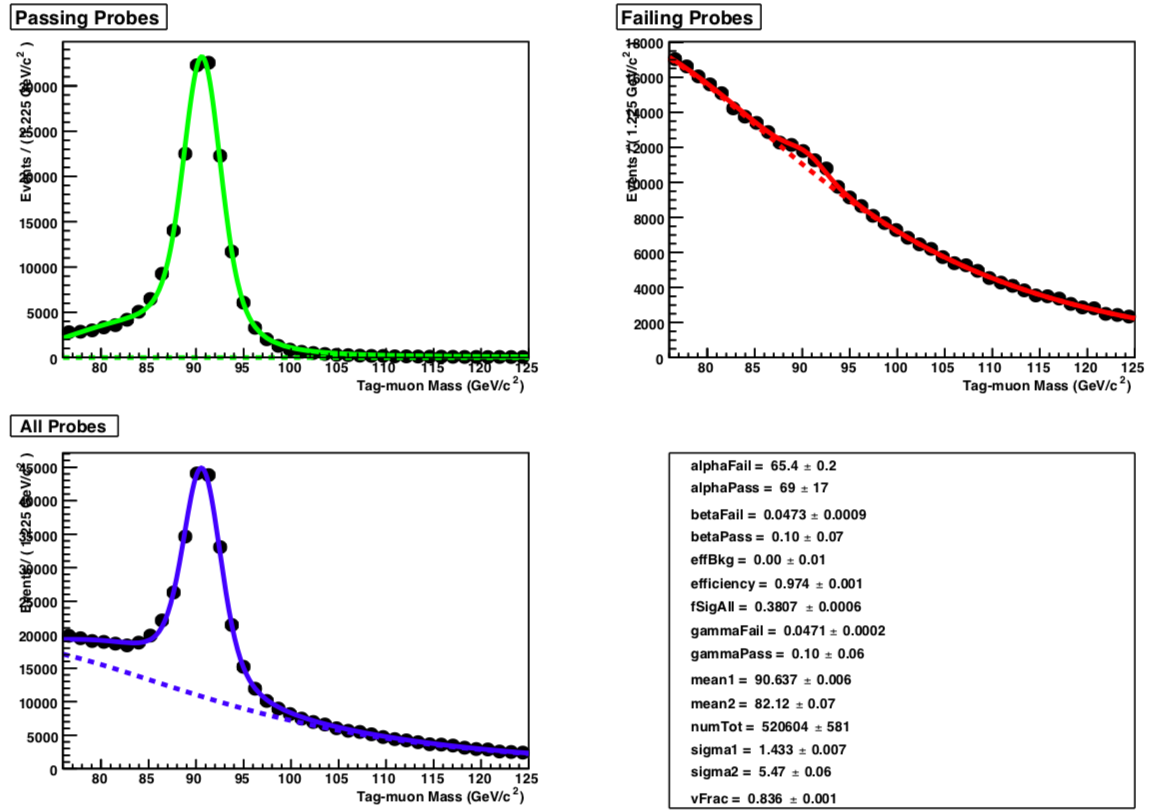
\includegraphics[width=0.9\linewidth]{figures/bg_tnpmuonid.png}
\caption{An example of one $p_T - \eta$ bin of the $\mu\mu$ invariant mass spectrum with the $signal+background$ fittings for the efficiency measurement of the Tracker High $p_T$ ID.}
\label{fig:bg_tnpmuonid}
\end{center}
\end{figure}

\vspace{0.3cm}
Figure~\ref{bg_muontkideff} to \ref{bg_muonmcideff} shows the efficiency results calculated from both Tracker High $p_T$ ID and High $p_T$ ID.

\begin{figure}[htbp]
\begin{center}
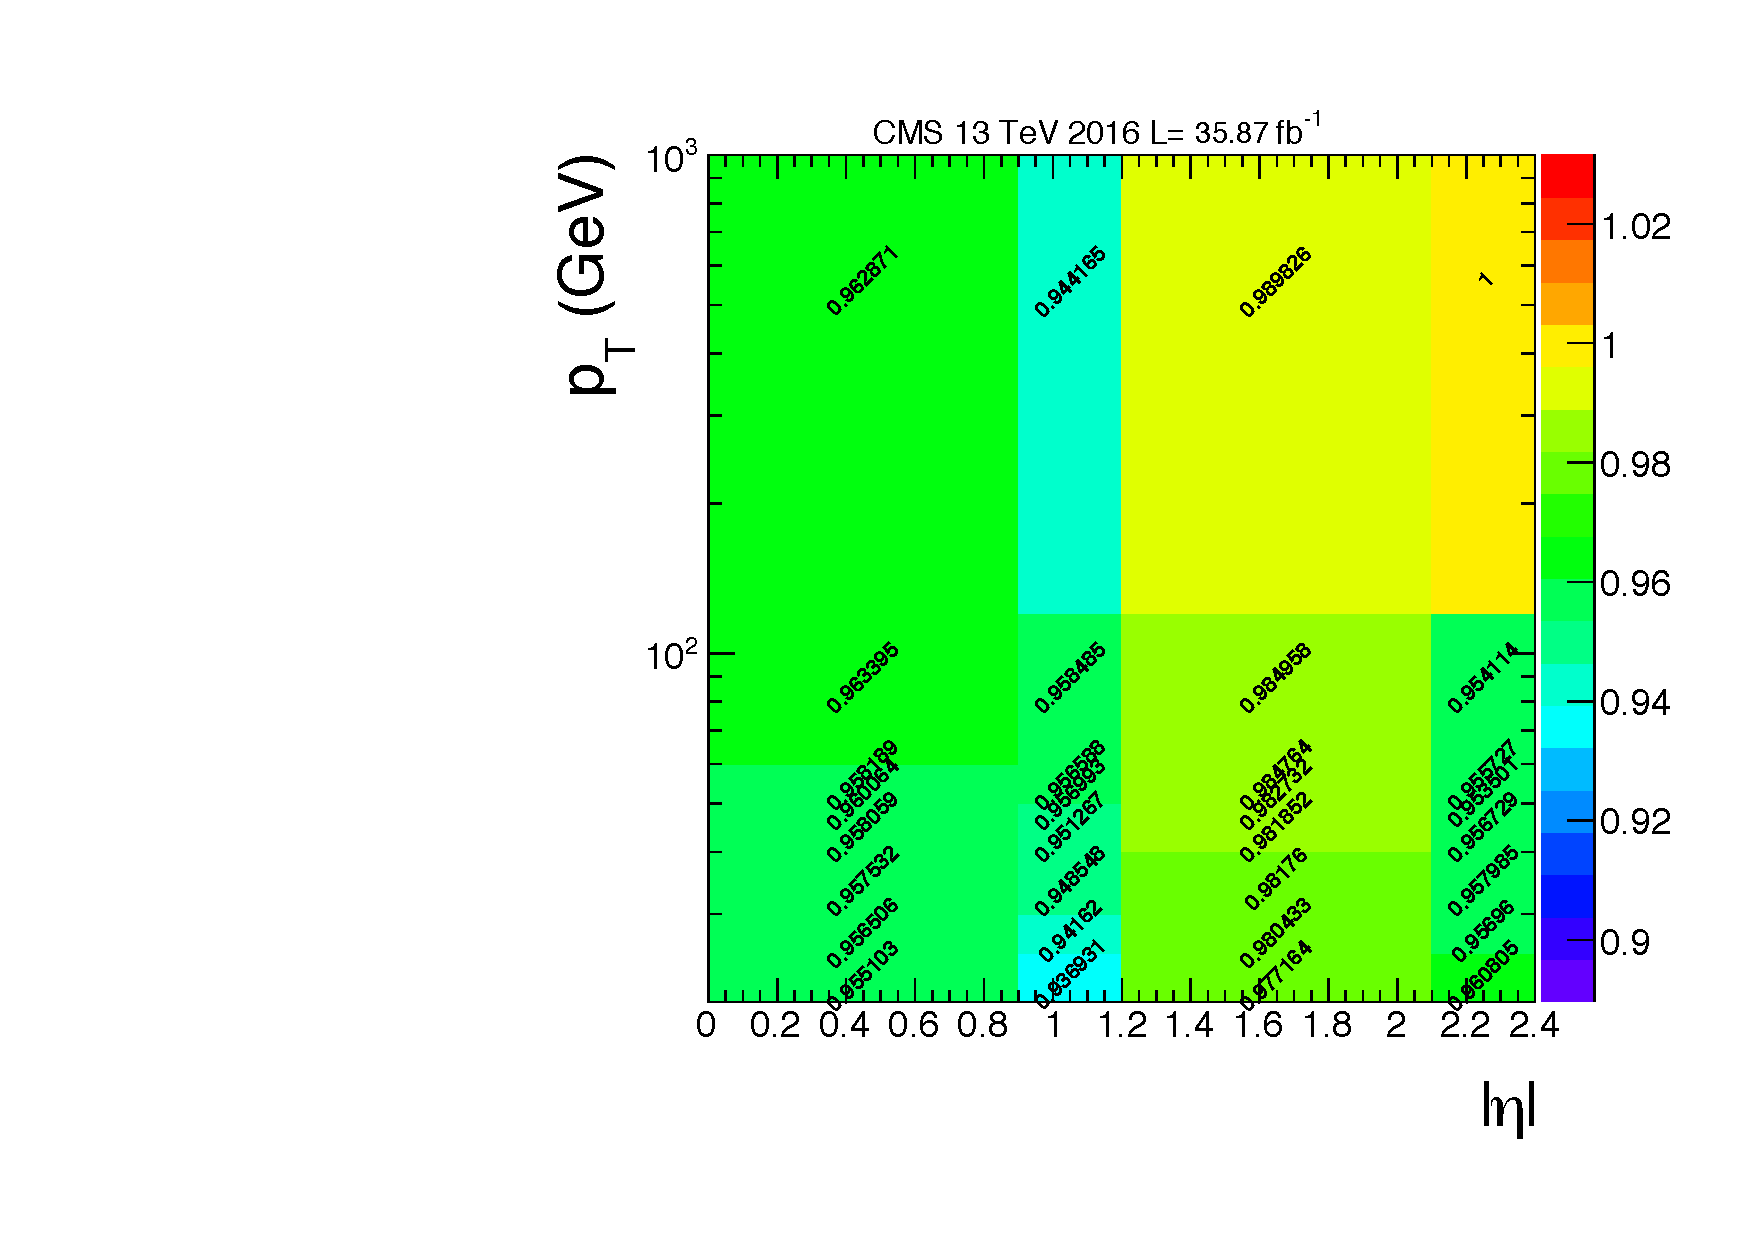
\includegraphics[width=0.49\linewidth, page=1]{figures/bg_muonidisoeff.pdf}
\includegraphics[width=0.49\linewidth, page=2]{figures/bg_muonidisoeff.pdf}
\caption{High $p_T$ Muon ID efficiency for 2016 ReReco data as a function of muon $p_T$ and $|\eta|$, for 2016 B-F (left) and 2016 GH (right).}
\label{fig:bg_muontkideff}
\end{center}
\end{figure}

\begin{figure}[htbp]
\begin{center}
\includegraphics[width=0.49\linewidth, page=3]{figures/bg_muonidisoeff.pdf}
\includegraphics[width=0.49\linewidth, page=4]{figures/bg_muonidisoeff.pdf}
\caption{Tracker High $p_T$ Muon ID efficiency for 2016 ReReco data as a function of muon $p_T$ and $|\eta|$, for 2016 B-F (left) and 2016 GH (right).}
\label{fig:bg_muonideff}
\end{center}
\end{figure}

\begin{figure}[htbp]
\begin{center}
\includegraphics[width=0.49\linewidth, page=5]{figures/bg_muonidisoeff.pdf}
\includegraphics[width=0.49\linewidth, page=6]{figures/bg_muonidisoeff.pdf}
\caption{Muon ID efficiency for RunIISummer16 MC as a function of muon $p_T$ and $|\eta|$, for High $p_T$ Muon ID (left) and Tracker High $p_T$ Muon ID (right).}
\label{fig:bg_muonmcideff}
\end{center}
\end{figure}

As the Tracker High $p_T$ ID is a loosen version of the High $p_T$ ID. if a muon passes the High $p_T$ ID, it would pass the Tracker High $p_T$ ID too. Then the muon ID scale factor for an event would be calculated as:
\begin{equation}
\epsilon^{data}/\epsilon^{MC} =\frac{(\epsilon_{HighPt}(\mu_1)\times \epsilon_{trkHighPt}(\mu_2)+\epsilon_{trkHighPt}(\mu_1)\times \epsilon_{HighPt}(\mu_2)-\epsilon_{HighPt}(\mu_1)\times \epsilon_{HighPt}(\mu_2))_{data}}{(\epsilon_{HighPt}(\mu_1)\times \epsilon_{trkHighPt}(\mu_2)+\epsilon_{trkHighPt}(\mu_1)\times \epsilon_{HighPt}(\mu_2)-\epsilon_{HighPt}(\mu_1)\times \epsilon_{HighPt}(\mu_2))_{MC}}
\end{equation}

\subsubsection{Muon Iso Efficiency}
The muon tracker isolation efficiency is also measured using the tag-and-probe method, with an additional requirment on the probe muon to pass the tracker High $p_T$ ID. As the tracker isolation selection applies to both muons, the ratio between the efficiencies of data and MC is calculated as the scale factor of the isolation. The SF values versus $p_T - \eta$ are show in Figure~\ref{fig:muonisosf}
\begin{figure}[htbp]
\begin{center}
\includegraphics[width=0.49\linewidth, page=7]{figures/bg_muonidisoeff.pdf}
\includegraphics[width=0.49\linewidth, page=8]{figures/bg_muonidisoeff.pdf}
\caption{\texttt{tracker ISO} data/MC efficiency scale factors a function of muon $p_T$ and $|\eta|$, for 2016 B-F (left) and 2016 GH (right).}
\label{fig:bg_muonisosf}
\end{center}
\end{figure}

\subsection{Electron ID/Iso Efficiency}
Based on the recommendation from EGamma POG, the \texttt{Loose} cut-based identification (ID) selection is required for all the electron candidates. As a PF isolation is already included in the \texttt{Loose} ID, no additional electron isolation is needed.

\vspace{0.3cm}
The electron \texttt{Loose} ID (including PF ISO) efficiency and scale factors are provided by the EGamma POG, measured by the tag-and-probe method. Figure~\ref{fig:bg_eidsf} shows the electron \texttt{Loose} ID scale factors from EGamma POG used in this analysis. The electron reconstruction is also affected by the tracking inefficiency issue, the reconstruction scale factors are also provided by the EGamma POG to counter this effect. Figure~\ref{fig:bg_gsfsf} shows the electron reconstruction scale factors from EGamma POG used in this analysis.  

\begin{figure}[htbp]
\centering
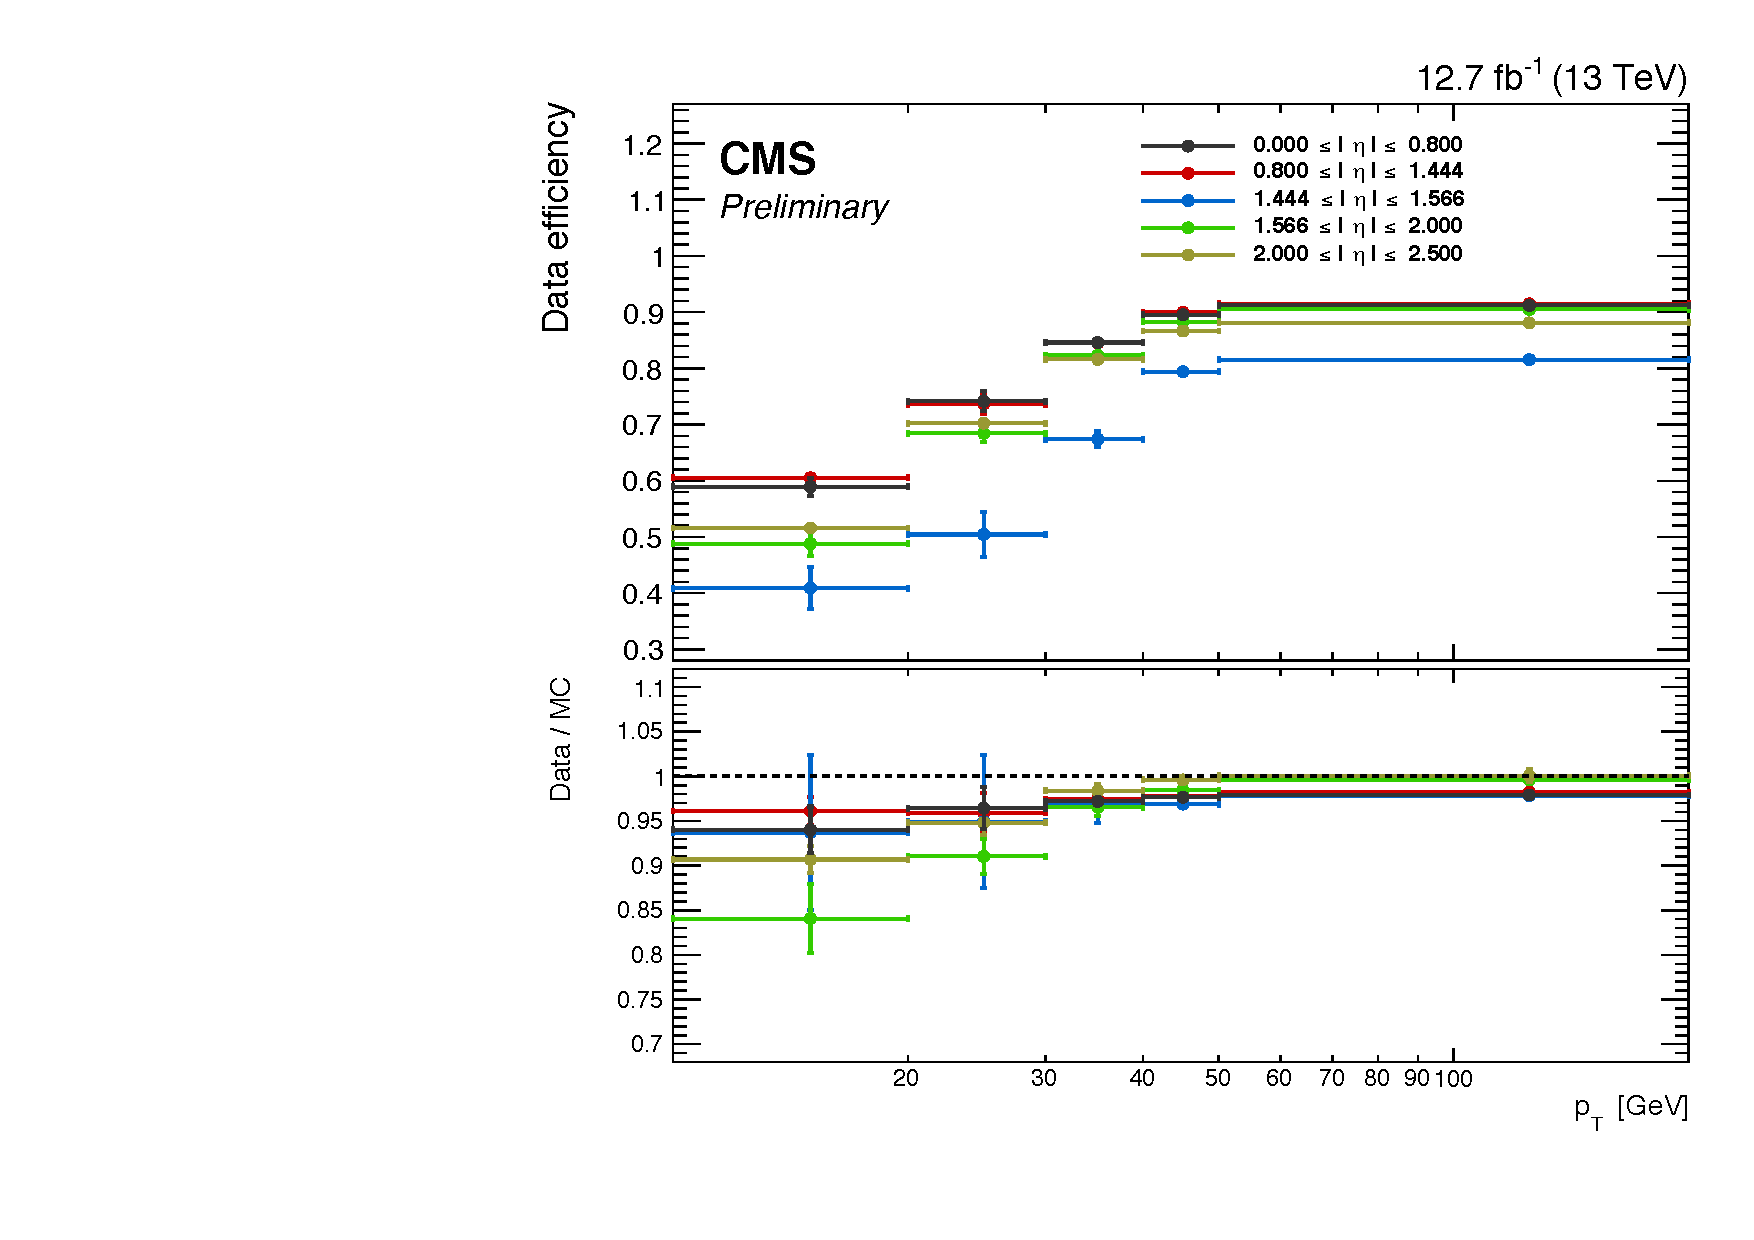
\includegraphics[width=0.66\linewidth, page=1]{figures/bg_elooseideff.pdf}
\includegraphics[width=0.66\linewidth, page=2]{figures/bg_elooseideff.pdf}
\caption{EGamma POG electron \texttt{Loose} ID (including pf Iso) efficiency scale factors for 2016 dataset analysis.}
\label{fig:bg_eidsf}
\end{figure}

\begin{figure}[htbp]
\centering
\includegraphics[width=0.66\linewidth, page=2]{figures/bg_erecoeff.pdf}
\caption{EGamma POG electron reconstruction scale factors for 2016 dataset analysis.}
\label{fig:bg_gsfsf}
\end{figure}

\subsection{Trigger Efficiency}\label{sec:bkg_trig}
The HLT is designed serving the purpose of fast decision making on data taking, and therefore the reconstruction of objects' properties on the HLT level are not precise enough compared to the offline reconstruction. Trigger efficiency study is important to physics analyses in two aspects: to suppress the trigger efficiency effect on the data by optimizing data selection; and to compensate the discrepancy in terms of trigger efficiency between data and simulation samples by applying trigger efficiency SFs to MC samples.
\subsubsection{SingleMuon HLT Efficiency}
For the muon channel selection, A event are required to pass the single muon HLT of either \texttt{HLT\_Mu50} or \texttt{HLT\_TkMu50}. The combined trigger efficiencies and SFs are centrally derived by the Muon POG, measured with the tag-and-probe method. The results are shown in Figure~\ref{fig:bg_trgeff_mu_dt}, \ref{fig:bg_trgeff_mu_mc}, and \ref{bg_fig:trgeff_mu_sf}.

\begin{figure}[htpb]
\begin{center}
\includegraphics[width=0.49\linewidth, page=1]{fig/muon_trg_summer16.pdf}
\includegraphics[width=0.49\linewidth, page=3]{fig/muon_trg_summer16.pdf}
\caption{Muon trigger efficiency from 2016 ReReco dataset as a function of reconstructed muon $p_T$ and $\eta$, for 2016 B-F (left) and 2016 GH (right). }
\label{fig:bg_trgeff_mu_dt}
\end{center}
\end{figure}

\begin{figure}[htpb]
\begin{center}
\includegraphics[width=0.49\linewidth, page=5]{fig/muon_trg_summer16.pdf}
\includegraphics[width=0.49\linewidth, page=7]{fig/muon_trg_summer16.pdf}
\caption{Muon trigger efficiency from  RunIISummer16 MC as a function of reconstructed muon $p_T$ and $\eta$,for 2016 B-F (left) and 2016 GH (right). }
\label{fig:bg_trgeff_mu_mc}
\end{center}
\end{figure}

\begin{figure}[htpb]
\begin{center}
\includegraphics[width=0.49\linewidth, page=9]{fig/muon_trg_summer16.pdf}
\includegraphics[width=0.49\linewidth, page=11]{fig/muon_trg_summer16.pdf}
\caption{Electron trigger efficiency Data/MC scale factors  as a function of reconstructed muon \pt and $\eta$, for 2016 B-F (left) and 2016 GH (right). }
\label{fig:bg_trgeff_mu_sf}
\end{center}
\end{figure}

\subsubsection{SingleElectron HLT Efficiency}
The SingleElectron HLT (\texttt{HLT\_Ele115\_CaloIdVT\_GsfTrkIdT}) is measured for data and MC using the tag-and-probe method. Events are selected from SingleElectron dataset for data and DYJetsToLL\_M-50\_TuneCUETP8M1\_13TeV-amcatnloFXFX-pythia8 dataset for MC with pileup reweight. The "tag" criteria are:
\begin{enumerate}
\item passing the \texttt{tight} cut-based identification (ID) and isolation (Iso) recommended by the EGamma POG %shown in Table~\ref{tab:electron-tightid}
\item passing \texttt{HLT\_Ele27\_WPTight\_Gsf} with $p_T>30$ and $|\eta|<2.1$
\end{enumerate}

%\begin{table}[htb!]
%  \center
%  \caption{The cuts used in the POG \texttt{tight} electron identification.}
%  \label{tab:electron-tightid}
%  \begin{tabular}{r c c c}
%    \hline
%    Variable & Barrel & Endcap \\
%    \hline
%    $|\eta_{\rm SC}|$ acceptance & $(0, 1.479)$ & $(1.479, 2.5)$\\
%    $\sigma_{i\eta,i\eta} <$ & 0.00998  & 0.0292 \\
%    $|\Delta\eta_{in}| <$ & 0.00308  & 0.00605 \\
%    $\Delta\phi_{in} <$ & 0.0816  & 0.0394 \\
%    \texttt{hOverE} $<$ & 0.0414  & 0.0641 \\
%    \texttt{relIsoWithEA} $<$ & 0.0588  & 0.0571 \\
%    $|1/E - 1/p| <$ & 0.0129  & 0.0129 \\
%    expectedMissingInnerHits $\leq$ & 1  & 1 \\
%    conversion veto & yes  & yes \\
%    \hline
%  \end{tabular}
%\end{table}

The criterion of \texttt{tight} ID/Iso ensures the tag electron to be a well defined electron. The \texttt{HLT\_Ele27\_WPTight\_Gsf} is the un-prescaled HLT with lowest $p_T$ threshold in the SingleElectron dataset, and ensures that the trigger efficiency to be measured from the probe electron would not be biased due to the dataset for selection. A electron would be considered as a probe if it satisfies the condition of the trigger efficiency measurement, which is passing the \texttt{loose} ID/Iso in this analysis.

\vspace{0.3cm}



\section{Zjets Background Modeling}\label{sec:dybk}

\section{Non-resonant Background Modeling}

\section{Irreducible Background Modeling}

\section{Control Plots}

\section{Plots in the Signal Region}
